


\usepackage{tikz}
\usetikzlibrary{arrows}
\usepackage{enumitem}
\usepackage{mathtools}
\usepackage{etoolbox}

\usepackage{amssymb}
\usepackage{amsmath}
\usepackage{framed}
\usepackage{pstricks}
\usepackage[framed]{ntheorem}


\mathtoolsset{centercolon} 
\DeclarePairedDelimiter\abs{\lvert}{\rvert}
\DeclarePairedDelimiter\ang{\langle}{\rangle}

%% my theorem styles
\newtheoremstyle{meng-margin}%
{\item[\hskip\labelsep {\bfseries ##1\ ##2}]}%
{\item[\llap{\itshape(##3)\quad\hskip\labelsep}  {\bfseries ##1\ ##2}]}%

\newtheoremstyle{meng-ex}%
{\item[\hskip\labelsep {\normalfont\bfseries ##1\ ##2}]}%
{\item[\hskip\labelsep {\normalfont\bfseries ##1\ ##2}\ {\itshape (##3)} ]}%

\newtheoremstyle{meng-thm}%
{\item[\hskip\labelsep {\normalfont\bfseries ##1\ ##2}]}%
{\item[\hskip\labelsep {\normalfont\bfseries ##1\ ##2}\ {\itshape (##3)} ]}%



%% exercise, example, definition
\theoremstyle{meng-ex}
\theorembodyfont{\normalfont\upshape}
\theoreminframepreskip{0pt}
\theoreminframepostskip{0pt}
\newtheorem{exercise}{Exercise}
\newtheorem{example}{Example}
\newframedtheorem{definition}{Definition}

\theoremstyle{meng-thm}
\theorembodyfont{\normalfont\itshape}
\theoremprework{\bigskip\hrule\leavevmode}
\theorempostwork{\hrule\leavevmode}
\newtheorem{theorem}{Theorem}
\newtheorem{lemma}{Lemma}
\newtheorem{corollary}{Corollary}



\DeclareMathOperator{\Aut}{Aut}
\DeclareMathOperator{\rot}{rot}
\def\IM{\text{Im}}
\def\inv{^{-1}}
\def\SL{\text{SL}_2(\mathbb R)}
\def\H{\mathbb{H}}
\def\D{\mathbb{D}}
\def\R{\mathbb{R}}
\def\C{\mathbb{C}}
\renewcommand{\vec}[1]{\mathbf{#1}}
\DeclarePairedDelimiterX\norm[1]\lVert\rVert{
	\ifblank{#1}{\:\cdot\:}{#1}
}



\usepackage{enumitem}
\def\labelenumi{\textbf{(\alph*)}}
\title{A Big (but now is small) List of Problems/Solutions}
\author{Meng Sivmeng}
\date{\today}

\begin{document}

\maketitle
\chapter{Complex Analysis}

\begin{problem}[Stien, Ex 1, p. 64]
  Prove that
  \[\int_{0}^{\infty}\sin(x^2)dx=\int_{0}^{\infty}\cos(x^2)dx=\frac{\sqrt{2\pi}}{4}.\]
\end{problem}
\begin{solution}
	Let $f(z)=e^{-z^2}$, and define $C$ to be the positively oriented closed contour
  as below:
  \begin{center}
  	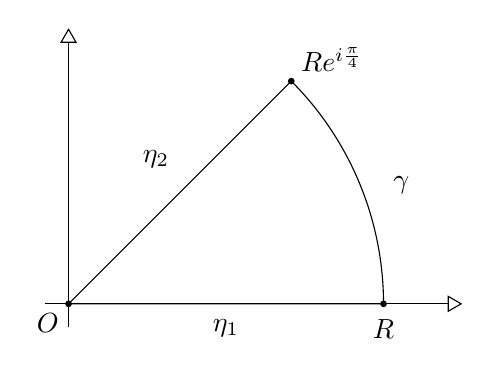
\begin{tikzpicture}
    	\draw[-open triangle 60] (-0.3, 0)--(5,0);
    	\draw[-open triangle 60] (0, -0.3)--(0,3.5);

      \draw (0,0)--(4,0)-- (4,0) arc [start angle=0, end angle=45, radius=4] --cycle;
      \draw[fill=black] (45:4) node[above right]{$Re^{i\frac{\pi}{4}}$} circle [radius=1pt] ;
      \draw[fill=black] (4,0) node[below=2pt]{$R$} circle [radius=1pt] ;
      \draw[fill=black] (0,0) node[below left]{$O$} circle [radius=1pt] ;

      \node[below=2pt]  at (2,0) {$\eta_1$};
      \node[above left] at (1.4,1.6) {$\eta_2$};
      \node[right]      at (4,1.5) {$\gamma$};
    \end{tikzpicture}
  \end{center}
  Observe the following:
  \begin{itemize}
  \item We parametrize $\gamma$ by $\gamma(\theta)=Re^{i\theta}$ for $\theta\in[0,\frac{\pi}{4}]$.
    Estimate the integral on $\gamma$ we get
    \begin{align*}
      \abs*{\int_{\gamma}f(z)dz}
      &\leq \int_{0}^{\frac{\pi}{4}} \abs*{f(Re^{i\theta})}\cdot \abs*{Rie^{i\theta}}d\theta\\
      &=\int_0^{\frac{\pi}{4}}e^{-R^2\cos2\theta}\cdot Rd\theta
    \end{align*}
    Next we want to bound $\cos 2\theta$ to some linear function, using Graphing software
    we can conclude that
    $\cos2\theta\geq \frac{\pi}{4}-\theta$ for $\theta\in[0,\frac{\pi}{4}]$.
    Hence,
    \begin{align*}
      \abs*{\int_{\gamma}f(z)dz}
      &\leq R\int_{0}^{\frac\pi 4}e^{R^2 (\theta-\frac\pi 4)}d\theta\\
      &=R\cdot\frac1{R^2}\left[e^{R^2 (\theta-\frac\pi 4)}\right]_{0}^{\frac\pi 4}\\
      &=\frac1{R}(1-e^{-R^2\frac\pi 4})\to 0\quad \text{as } R\to\infty
    \end{align*}

    
  \item Let $\eta_3$ be the reverse of $\eta_2$, i.e. we can
    parametrize $\eta_3$ as $\eta_3(t)=te^{i\frac\pi 4}$ for
    $t\in [0,R]$, and thus
    \begin{align*}
      \int_{\eta_2}f(z)dz
      & = -\int_{\eta_3} f(z)dz\\
      & = -\int_{0}^{R} e^{-t^2e^{i\frac\pi 2}}\cdot e^{i\frac\pi 4} dt\\
      & = -e^{i\frac\pi 4}\int_{0}^{R}e^{-ix^2}dx
    \end{align*}
  \end{itemize}
  Since $f$ is holomophic there, by Cauchy's theorem we obtain
  \begin{align*}
  	\oint_C f(z)dz=
    \int_{\eta_1}f(x)dx + \int_{\eta_2}f(z)dz + \int_{\gamma}f(z)dz=0
  \end{align*}
  Now, taking the limit as $R\to\infty$, we obtain
  \begin{align*}
  	&\int_0^{\infty}e^{-x^2}dx+0-e^{i\frac\pi 4}\int_0^\infty e^{-ix^2}dx=0\\\implies\quad
    &\int_0^{\infty}[\cos(x^2)-i\sin(x^2)]dx = e^{-i\frac\pi 4}\cdot \frac{\sqrt\pi}2
  \end{align*}
  Therefore,
  \[
    \boxed{\int_{0}^{\infty}\cos(x^2)dx=\int_{0}^{\infty}\sin(x^2)dx=\frac{\sqrt{2\pi}}{4}}
  \]
\end{solution}




\begin{problem}[Stien, Ex 2, p. 64]
	Show that $\displaystyle\int_0^{\infty}\frac{\sin x} xdx=\frac\pi 2$.
\end{problem}
\begin{solution}
	From the hint in the book, observe that
  \begin{align*}
  	\frac1{2i}\int_{-\infty}^{\infty}\frac{e^{ix}-1}x dx
    &=\frac1{2i}\int_{-\infty}^{\infty}\frac{\cos x-1 +i\sin x}x dx\\
    &=\frac1{2i}\int_{-\infty}^{\infty}\frac{\cos x-1}{x}dx +
      \frac1{2}\int_{-\infty}^{\infty}\frac{\sin x}x dx
  \end{align*}
  Since $\frac{\cos x-1}x$ is an odd function, and
  $\frac{\sin x}x$ is an even function, we conclude that
  \[
    \boxed{
    \frac1{2i}\int_{-\infty}^{\infty}\frac{e^{ix}-1}x dx
    = \int_{0}^{\infty}\frac{\sin x}x dx}
  \]
  Now let $f(z)=\frac{e^{iz}-1}{z}$, and the indented circle $C$ as below
  \begin{center}
    \begin{tikzpicture}

    	\draw (4,0) arc [start angle=0, end angle=180, radius=4];
    	\draw (0.5,0) arc [start angle=0, end angle=180, radius=0.5];
      \draw (-4,0)--(-0.5,0) (0.5,0)--(4,0);

      \node[below=2pt] at (-4,0)   {$-R$};
      \node[below=2pt] at (-0.5,0) {$-\epsilon$};
      \node[below=2pt] at (0.5 ,0) {$\epsilon$};
      \node[below=2pt] at ( 4,0)   {$R$};
    \end{tikzpicture}
  \end{center}
  Let $\gamma_{\epsilon}$ and $\gamma_{R}$ be the positively oriented semi circle
  centered at $O$ with radii $\epsilon$ and $R$ respectively.
  \begin{itemize}
  \item Using series expansion of $e^z$ reveals that
    $\displaystyle\lim_{z\to 0}\frac{e^{iz}-1}{z}=i$, so if we set $f(0)=i$ we obtain
    that $f$ is continuous around $z=0$. Hence $f$ is bounded
    there. Estimate the integral over $\gamma_{\epsilon}$
    \begin{align*}
    	\abs*{\int_{\gamma_\epsilon}f(z)dz}
      &\leq \sup_{z\in\gamma_\epsilon}\abs{f(z)}\cdot \text{length}(\gamma_\epsilon)\\
      &\leq M\cdot \pi\epsilon
    \end{align*}
    hence this integral approaches to $0$ as $\epsilon\to 0$.

    
  \item For $\gamma_R$,
    \[
      \int_{\gamma_R}f(z)dz = \int_{\gamma_R}\frac{e^{iz}}{z}dz - \int_{\gamma_R}\frac1{z}dz
    \]
    but
    \begin{align*}
    	\abs*{\int_{\gamma_R}\frac{e^{iz}}{z}dz}
      &\leq \int_{0}^{\pi}\abs*{
        \frac{e^{iRe^{i\theta}}}{Re^{i\theta}}}\cdot \abs*{Rie^{i\theta}}d\theta\\
      &=\int_0^\pi e^{-R\sin\theta}d \theta = 2\int_{0}^{\frac\pi 2}e^{-R\sin\theta}d \theta
    \end{align*}
    From Jordan's inequality, $\sin\theta\geq\frac{2\theta}{\pi}$
    for $\theta\in[0,\frac\pi 2]$, then
    \begin{align*}
    	\abs*{\int_{\gamma_R}\frac{e^{iz}}{z}dz}
      &\leq\int_0^{\frac\pi 2}e^{-R\frac{2\theta}\pi} d\theta\\
      &=-\frac{\pi}{2R}\Big[e^{-R\frac{2\theta}\pi}\Big]_{0}^{\frac\pi 2}\\
      &=-\frac{\pi}{2R}\cdot (e^{-R}-1)\to 0\quad\text{as } R\to\infty
    \end{align*}
  \end{itemize}
  Because $f$ is holomorphic on and inside $C$, apply Cauchy's theorem and letting
  $R\to\infty$ and $\epsilon\to 0$, we obtain
  \begin{align*}
  	&\int_{-R}^{-\epsilon}f(x)dx+\int_{\epsilon}^{R}f(x)dx
      - \int_{\gamma_\epsilon}f(z)dz + \int_{\gamma_R}f(z)dz = 0\\\implies\quad
    &\int_{e\leq\abs{x}\leq R}f(x)dx =
      \int_{\gamma_\epsilon}f(z)dz
      -\int_{\gamma_R}\frac{e^{iz}}{z}
      +\int_{\gamma_R}\frac1{z}dz\\\implies\quad
    &\int_{-\infty}^{\infty}\frac{e^{ix}-1}{x}dx = 0 - 0 + i\pi \\\implies\quad
    &\int_{0}^{\infty}\frac{\sin x}{x}dx = \frac1{2i}\int_{-\infty}^{\infty}\frac{e^{ix}-1}{x}dx
      = \boxed{\frac\pi 2}.
  \end{align*}
\end{solution}

\begin{problem}[Stein, Ex 7, p. 65]
	Suppose $f:\mathbb D\to\C$ is holomorphic. Show that the diameter
  $d=\sup_{z,w\in\mathbb D}\abs{f(z)-f(w)}$ of the image f $f$
  satisfies
  \[2\abs{f'(0)}\leq d.\]
\end{problem}
\begin{solution}
	Let $0<r<1$. From Cauchy formula
  \[f'(0)=\frac1{2\pi i}\int_{C_r}\frac{f(z)}{z^2}dz.\]
  Let $g(z)=-f(-z)$, we then have
  \[
    \frac1{2\pi i}\int_{C_r}\frac{-f(-z)}{z^2}dz
    =\frac1{2\pi i}\int_{C_r}\frac{g(z)}{z^2}dz
    =g'(0)=f'(0)
  \]
  Adding these two quantities,
  \begin{align*}
    2f'(0)
    &= \frac1{2\pi i}\int_{C_r}\frac{f(z)-f(-z)}{z^2}dz\\ \implies\quad
    2\abs{f'(0)}
    &\leq \frac1{2\pi}\sup_{z\in\mathbb D}\abs*{\frac{f(z)-f(-z)}{z^2}}\cdot 2\pi r\\
    &\leq \frac1r \sup_{z\in\mathbb D}\abs{f(z)-f(-z)}\leq \frac dr
  \end{align*}
  Thus $2\abs{f'(0)}$ is a lower bound of $\{\frac dr:0<r<1\}$, therefore
  \[
    2\abs{f'(0)}\leq\inf_{0<r<1}\frac dr = d
  \]
\end{solution}


%% =======================================================
\begin{problem}[Stien, Ex 2, p. 103]
  Evaluate the integral
  \[
    \int_{-\infty}^{\infty}\frac{dx}{1+x^4}.
  \]
\end{problem}
\begin{solution}
	Consider the integral of the function
  $f(z)=\frac1{1+z^4}$ over the contour $C$ as below:

  \begin{center}
  	\begin{tikzpicture}
    	\draw[-open triangle 60] (-0.3, 0)--(5,0);
    	\draw[-open triangle 60] (0, -0.3)--(0,5);

      \draw (4,0) -- (4,0) arc[start angle=0, end angle=90, radius=4];
      \draw[fill=black] (45:2)node[above right]{$e^{i\frac\pi 4}$} circle[radius=1pt]; 
    \end{tikzpicture}
  \end{center}
  \begin{itemize}
  \item 
    The point $z_0=e^{i\frac\pi 4}$ is a simple pole of $f$ and its residue is
    \[
      \text{res}_{z_0}
      =\lim_{z\to z_0}\frac{z-z_0}{1+z^4}
      =\lim_{z\to z_0}\frac{1}{4z^3}=\frac1{4e^{i\frac{3\pi}{4}}}
    \]

  \item Let $\gamma_1$ be the line from $O$ to $R$, and we let
    \[I_R=\int_{0}^{R}\frac1{1+x^4}dx\]
  \item Let $\gamma_2$ be the above arc, observe that
    \[
      \abs*{\int_{\gamma_2}f(z)dz}
      \leq \frac\pi 2R\cdot\sup_{z\in\gamma_2}\abs*{\frac1{1+z^4}}
      \leq \frac\pi 2R\cdot\frac1{R^4-1}\to 0
    \]
    as $R\to\infty$.

    
  \item Let $\gamma_3$ be the line from $O$ to $iR$ and we can parametrize
    it as $t\mapsto it$ when $t\in[0,R]$. Thus the integral
    \begin{align*}
    	\int_{\gamma_3}f(z)dz = \int_0^R \frac{1}{1+(it)^4}\cdot idt = iI_R
    \end{align*}
  \end{itemize}
  Applying Cauchy theorem
  \begin{align*}
  	\oint_C f(z)dz =
    \int_{\gamma_1}f(z)dz+
    \int_{\gamma_1}f(z)dz-
    \int_{\gamma_1}f(z)dz=2\pi i\cdot\text{res}_{z_0}
  \end{align*}
  Letting $R\to\infty$, we obtain that
  \begin{align*}
  	&(1-i)I = 2\pi i\cdot \frac{e^{-i\frac{3\pi}4}}{4}
    \\\implies\quad
    &I = \frac{\pi i}{2\sqrt 2}e^{-i\frac{3\pi}4}\cdot e^{i\frac{\pi}4}
      =\frac\pi {2\sqrt 2}.
    % &\int_{0}^{\infty}\f(x)dx = \frac{\pi i}{2\sqrt 
  \end{align*}
  Because $\frac1{1+x^4}$ is an even function we get
  \[\int_\{-\infty\}^{\infty}f(x)dx=2\int_{0}^{\infty}\frac1{1+x^4}=\frac\pi 2.\]
\end{solution}

\begin{problem}[Stien, Ex 3, p. 103]
	Show that
  \[
    \int_{-\infty}^{\infty}\frac{\cos x}{x^2+a^2}dx =
    \pi\frac{e^{-a}}{a},\qquad \text{for $a>0$.}
  \]
\end{problem}
\begin{solution}
	We integrate the function $f(z)=\frac{e^{iz}}{z^2+a^2}$ along with the semi-circle
  shown below. In this contour, $f$ has a simple pole at $z=ia$. The residue correspond
  to this pole is
  \[
    \text{res}_{ia} = \lim_{z\to ia}\frac{e^{iz}}{z+ia}=\frac{e^{-a}}{2ia}
  \]

  \begin{center}
    \begin{tikzpicture}[scale=0.8]
    	\draw[-open triangle 60] (-5, 0)--(5,0);
    	\draw[-open triangle 60] (0, -0.3)--(0,5);

      \draw (4,0) -- (4,0) arc[start angle=0, end angle=180, radius=4];
      \draw[fill=black] (0,2.5)node[right]{$ia$} circle[radius=1pt]; 
    \end{tikzpicture}
  \end{center}
  By Estimation theorem, the integral along the upper arc
  \begin{align*}
    \abs*{\int_{\text{arc}} f(z)dz }
    &\leq \pi R\cdot\sup_{z\in\text{arc}}\abs*{\frac{e^{iz}}{z^2+a^2}}\\
    &\leq \pi R\cdot\sup_{\theta\in[0,\pi]}\frac{e^{-R\sin\theta}}{R^2-a^2}
  \end{align*}
  And as $R\to\infty$, the RHS approaches to zero. Thus the integral is also zero.
  Now applying Cauchy's residue theorem and let $R\to\infty$, we obtain that
  \begin{align*}
    &\int_{-R}^{R}f(x)dx + \int_{\text{arc}}f(z)dz = 2\pi i\cdot\text{res}\\\implies\quad
    &\int_{-\infty}^{\infty}\frac{\cos x+i\sin x}{x^2+a^2} dx = 2\pi i\cdot\frac{e^{-a}}{2ia}\\
    \implies\quad
    &\int_{-\infty}^{\infty}\frac{\cos x}{x^2+a^2}dx = \pi\cdot\frac{e^{-a}}{a}
  \end{align*}
\end{solution}


\begin{problem}[Stien, Ex 6 p. 104]
	Show that
  \[\int_{-\infty}^{\infty}\frac{dx}{(1+x^2)^{n+1}}dx = \frac{(2n-1)!!}{(2n)!!}\cdot\pi. \]
\end{problem}
\begin{solution}
	We integrate the function $f(z)=\frac{1}{(1+z^2)^{n+1}}$ along with the semi-circle
  shown below. In this contour, $f$ has a pole of oder $n+1$ at $z=i$. The residue correspond
  to this pole is
  \begin{align*}
    \text{res}_{i}
    &= \lim_{z\to i}\frac1{n!}\frac{d^n}{dz^n}(z+i)^{-n-1}\\
    &= \lim_{z\to i}\frac1{n!}(-n-1)(-n-2)\cdots(-n-n)(z+i)^{-2n-1}\\
    &= \frac1{n!}(-1)^n(n+1)(n+2)\cdots (2n)\frac1{(2i)^{2n+1}}\\
    &=\frac1{n!2^n}\cdot\frac{(n+1)(n+2)\cdots(2n)}{2^n}\cdot\frac{(-1)^n}{2i^{2n}i}\\
    &=\frac1{(2n)!!}\cdot (2n-1)!!\cdot\frac1{2i}
  \end{align*}

  \begin{center}
    \begin{tikzpicture}[scale=0.8]
    	\draw[-open triangle 60] (-5, 0)--(5,0);
    	\draw[-open triangle 60] (0, -0.3)--(0,5);

      \draw (4,0) -- (4,0) arc[start angle=0, end angle=180, radius=4];
      \draw[fill=black] (0,2.5)node[right]{$i$} circle[radius=1pt]; 
    \end{tikzpicture}
  \end{center}
  Applying Cauchy Residue Theorem,
  \begin{align*}
  	&\int_{-R}^{R}f(x)dx + \int_{\text{arc}}f(z)dz = 2\pi i\cdot\text{res}
      \intertext{
      Letting $R\to\infty$ and arguing as above, we found that the integral
      along the arc is zero, hence
      }
      \implies\quad
    &\int_{-\infty}^{\infty}f(x)dx + 0 =2\pi i\cdot \frac{(2n-1)!!}{(2n)!!}\cdot\frac1{2i} \\
    \implies\quad
    &\boxed{\int_{-\infty}^{\infty}\frac1{(1+x^2)^{n+1}}dx = \frac{(2n-1)!!}{(2n)!!}\cdot \pi}
  \end{align*}
\end{solution}



\end{document}    
